% Исходный LaTeX-код (c) Пётр Калинин
% Код распространяется по лицензии GNU GPL (!)

\header{Поиск в глубину для ориентированных графов: топологическая сортировка и смежные вопросы}

На первый взгляд может показаться, особенно после прочтения первой части этого текста, что поиск в 
глубину для \textit{ориентированных} графов ничего хорошего не даст. Но это не так. 
Как ни странно, но ориентированные графы "--- пожалуй, наиболее часто используемая арена для поиска 
в глубину. В частности, топологическая сортировка ациклического графа очень часто бывает нужна, 
наверное, намного чаще, чем проверка графа на двудольность/на дерево...

В общем, в этом разделе мы будем рассматривать ориентированные графы.

\lheader{Топологическая сортировка}
\textit{Ациклическим} называется ориентированный граф, в котором нет (ориентированных, конечно) 
циклов. 
\taskn{Контрольный вопрос}|Понимаете ли вы, что этот класс намного шире, чем деревья? Т.е.
что ациклический граф "--- это не только ориентированное дерево?||||Ясно, что могут быть ациклические графы "--- не деревья. Например, три вершины и 
ребра $1\to 2$, $1\to 3$ и $2\to 3$. Если снимем ориентацию с рёбер, то могут появиться циклы,
которых раньше не было из"=за того, что ребра были ориентированы.|\label{acyclicnontree}

Самая основная задача, которая может быть поставлена на ациклических графах "--- это 
\textit{топологическая сортировка} (сокращённо топсорт) такого графа. Несмотря на страшное 
название, на самом деле это 
просто. Задача состоит в том, чтобы пронумеровать вершины графа так, чтобы все ребра шли из вершин 
с меньшим номером в вершину с б\'{о}льшим. Или, говоря по"=другому, расположить вершины на прямой 
так, чтобы все ребра шли слева направо. Классическая легенда задачи гласит: есть $N$ дел, которые 
надо сделать. При этом про каждое дело известно, какие дела надо сделать обязательно \textit{до} 
него (и, соответственно, известно, какие надо сделать \textit{после}). Требуется определить 
порядок, в котором нужно делать эти дела.

Очевидно, что, если в графе есть циклы, то задача решения не имеет. Оказывается, если циклов нет, 
то задача имеет решение; как вы уже, наверное, догадались, доказывать мы это будем предъявлением 
соответствующего алгоритма.

На самом деле есть \textit{два} довольно существенно разных алгоритма решения этой задачи. Первый 
вообще не использует идеи поиска в глубину%
\footnote{Ну, конечно, можно, наверное, найти какие-нибудь идейные сходства у этих двух алгоритмов, и даже, 
может быть, можно, сильно помучившись, попытаться объявить, что в каком-то смысле они 
одинаковы\dots Но, может быть, это вообще верно для \textit{любых} двух решений одной и той же 
задачи? :)}%
, довольно очевиден идейно, но не очень тривиален в 
реализации. Он приведён в "<Искусстве программирования для ЭВМ"> Кнута и потому я буду называть его 
методом Кнута (он используется редко, и я не знаю, есть ли у него стандартное название. Кстати, когда говорят
"<алгоритм топологической сортировки">, обычно понимают не этот, а второй). Состоит этот алгоритм в следующем: 
в любом ациклическом графе точно есть "<сток">, т.е. вершина, из которой не выходит ни одного ребра 
(т.е. вершина, у которой \textit{исходящая степень} равна нулю). Очевидно, её можно поставить 
последней. После этого как бы мы ни ставили остальные вершины,  проблем с рёбрами, идущими в 
\textit{эту} вершину, не возникнет: они в любом случае будут идти направо. Тогда эту вершину вместе 
со всеми входящими в неё рёбрами (а исходящих, мы помним, нет) можно выкинуть из графа. 
Получившийся граф также будет ациклическим, и в нем тоже обязательно будет сток. Поставим его на 
предпоследнее место в массиве и выкинем из графа. И так далее. Очевидно, что в итоге все получится: 
поскольку каждую вершину мы ставили только тогда, когда она становилась стоком, то проблем ни с 
какими рёбрами не получится.

Кстати, я надеюсь, очевидно, почему в любом ациклическом графе обязательно найдётся сток? Если его 
нет, то встанем в произвольную вершину. Из неё есть выходящее ребро "--- пойдём по нему. Дальше 
опять найдётся выходящее ребро "--- и т.д. Гулять по графу мы сможем до бесконечности, а это 
обозначает, что вершины обязательно повторятся "--- найдётся цикл. Противоречие.

Таким образом, алгоритм: находим какой"=нибудь сток, ставим его на последнее место в выходном 
массиве, выкидываем его (а на самом деле просто помечаем в соответствующем массиве, что он выкинут, и 
в будущем при расчёте исходящей степени не учитываем его). Дальше находим новый сток и т.д., пока 
не расставим все вершины. Если на очередном шагу стока не найдётся, значит, граф не ациклический.
Заметьте, что мы таким образом доказали, что любой ациклический граф можно оттопсортить.

В простейшей реализации этот алгоритм будет работать за $O(V^3)$: действительно, каждый поиск стока 
занимает $O(V^2)$: перебрать все вершины и для каждой посчитать исходящую степень "--- а таких 
поисков надо сделать $V$. Но можно на самом деле все ускорить, и в итоге получить программу, 
работающую за $O(E)$ (как всегда, при условии, что граф хранится списком смежных вершин).

\task|Напишите эту программу. Попробуйте придумать, как можно заставить её работать быстрее. На 
самом деле это делается в два этапа: во"=первых, заметим, что каждый раз пересчитывать исходящую 
степень не надо, а на втором этапе вам пригодится структура данных очередь или стек. Попробуйте придумать 
это сами. Если не придумаете, то смотрите подсказки, которые есть по этому заданию (впрочем, как и 
по некоторым другим). Обязательно потом прочитайте подсказки и ответ; в частности, там будет пример
хранения графа списком смежных вершин.||Идея номер один состоит в следующем: будем в отдельном массиве для каждой вершины хранить 
её текущую исходящую степень. Тогда при удалении вершины будет достаточно пробежаться по всем входящим
в неё рёбрам и уменьшить на единицу исходящую степень соответствующих вершин; сами исходящие ребра можно не
удалять и даже не хранить (храним только входящие). Сток искать тогда можно просто пробегаясь по этому массиву и ища 
в нем нули.
Идея два состоит в том, чтобы, в добавок ко всему вышесказанному, хранить все стоки в отдельном массиве 
(по принципу стека, например). Когда
мы уменьшаем исходящую степень очередной вершины, то посмотрим: если степень стала нулевой, то вершина стала стоком
и мы её заносим в этот массив. Теперь не надо на каждом шагу пробегаться по всему массиву степеней в поисках нулей
"--- у нас есть отдельный массив, в котором хранятся вершины с нулевой исходящей степенью. Реализация и дополнительные комментарии 
в ответах (но сначала попробуйте сами написать!).||Приведу код, только сначала несколько комментариев про хранение графа списком смежных
вершин. Буду использовать настоящие списки, т.е.%
\footnote{Замечу, что это очень синтаксически странная конструкция: я использую идентификатор $pv$ до того,
как объяснил, что он значит. Паскаль такое допускает при выполнении двух условий: во"=первых, все должно быть в одной 
"<секции"> \texttt{type}, во"=вторых, должен быть определённый порядок: то ли сначала определён $tv$, потом $pv$,
то ли наоборот, я сейчас точно не помню. Если этот код не компилится, поменяйте их местами.}
\begin{codesample}\begin{verbatim}
type tv=record
          v:integer;
          next:pv;
       end;
     pv=^tv;
var gr:array[1..maxN] of pv;
\end{verbatim}
\end{codesample}
Здесь $tv$ "--- очередной элемент списка, хранящий одно ребро (т.е. одну смежную вершину):. $v$ "---
номер этой вершины, $pv$ "--- указатель на следующее ребро (на следующий элемент типа $tv$), или $nil$,
если такого ребра нет.
$gr$ хранит граф: для каждой вершины "--- указатель на первое ребро, \textit{в}ходящее в эту вершины (или $nil$,
если таких рёбер нет).

В данной задаче мы будем хранить только входящие ребра, т.к. исходящие нам не нужны (я говорил об этом
в подсказке). В других случаях для ориентированного графа могут понадобиться два массива отдельно для
входящих и исходящих рёбер; для неориентированного графа, конечно, нужен один массив.

Алгоритм:
\begin{codesamplec}{3}\begin{verbatim}
...
var st:array[1..maxN] of integer;
    nst:integer;
    d:array[1..maxN] of integer;
    u,v:integer;
    n,m:integer;
    nv:pv;
    ans:array[1..maxN] of integer;
    pos:integer;
    
begin
...
fllchar(gr,sizeof(gr),0);
fillchat(d,sizeof(d),0);
read(f,n,m);
for i:=1 to m do begin
    read(f,u,v);
    new(nv);
    nv^.v:=u;
    nv^.next:=gr[v];
    gr[v]:=nv;
    inc(d[u]);
end;
nst:=0;
for i:=1 to n do
    if d[i]=0 then begin
       inc(nst);
       st[nst]:=i;
    end;
pos:=n;
for i:=1 to n do begin
    {должно быть nst>0}
    v:=st[nst];
    dec(nst);
    ans[pos]:=v;
    dec(pos);
    nv:=gr[v];
    while nv<>nil do begin
          dec(d[nv^.v]);
          if d[nv^.v]=0 then begin
             inc(nst);
             st[nst]:=nv^.v;
          end;
          nv:=nv^.next;
    end;
end;
\end{verbatim}
\end{codesamplec}
$st$ "--- массив (стек) стоков; $nst$ "--- количество элементов в нем (т.е. количество стоков в текущем графе).
$d$ "--- массив исходящих степеней (т.е. $d[i]$ "--- исходящая степень $i$"=ой вершины). $ans$ "--- массив"=ответ,
$pos$ "--- позиция в этом массиве, куда мы должны будем поставить очередную вершину.

Сначала считываем граф. Я специально привожу этот текст, чтобы вы видели, как хранить граф списком смежных вершин.
Считаем, что граф задан списком рёбер: т.е. во входном файле сначала количества вершин ($n$) и рёбер ($m$), а потом 
по два числа на строке, задающие две вершины "--- откуда и куда идёт ребро. Поэтому считываем сначала эти количества,
а потом сами ребра. Каждое ребро $u\to v$ надо добавить в список рёбер, входящих в вершину $v$, т.е. в список $gr[v]$.
Посмотрите, как это делается. Тут небольшая путаница с тем, что ребро идёт из вершины $u$, поэтому приходится
писать $nv.v:=u$, но это мелочи. Может быть, можно было придумать более хорошие имена полям и переменным. Обратите
внимание, что, как всегда при вставке в список, мы вставляем в его начало, а не в конец. Заодно параллельно
считаем в массиве $d$ исходящие степени.

После этого формируем начальный список стоков $st$, пробегаясь по массиву $d$ и ища там нули. 

Далее основная часть. Мы должны $n$ раз подряд взять сток, поставить его в выходной массив и удалить его из графа.
Каждый раз сток точно найдётся, т.к. граф ациклический, поэтому все время должно быть $nst>0$. Берём очередной сток
(конечно, последний из массива $st$ "--- его проще удалять, чем первый), удаляем его из массива $st$ (командой
$dec(nst)$ просто), ставим в выходной массив и пробегаемся по входящим рёбрам, обратите внимание как. Для каждого
ребра просто уменьшаем на единицу исходящую степень соответствующей вершины и, если она стала стоком, заносим её
в массив $st$. Частая ошибка здесь "--- забыть написать \verb'nv:=nv^.next', чтобы перейти к следующему ребру. Это вам не
for, который переменную цикла автоматически увеличивает.|\label{Knuthalgorithm}

Кстати, замечу, что, очевидно, вместо стоков можно точно также использовать истоки "--- вершины, у 
которых \textit{входящая} степень равна нулю, и вообще, задача топологической сортировки обладает 
соответствующей симметрией: если обратить все ребра, то искомый порядок вершин тоже просто 
обратится.

Вышеприведённый алгоритм на самом деле очень интересен, а две идеи его ускорения весьма красивы. Но 
перейдём ко второму алгоритму, который напрямую использует поиск в глубину. Давайте, как и в первом 
алгоритме, будем заполнять выходной массив справа налево, т.е. от б\'{о}льших номеров к меньшим. 
Подумаем, когда можно поставить некоторую вершину? Очевидно, лишь после того, как поставлены все 
вершины, в которые из нашей идут ребра. Получаем следующую процедуру, ставящую вершину $i$ в 
выходной массив: 
\begin{center}
перебрать все выходящие из $i$ ребра и поставить в выходной массив вершины, в 
которые эти ребра идут. После этого поставить нашу. 
\end{center}
Но как мы будем ставить эти самые вершины, "<в которые эти ребра идут">? Очевидно, 
\textit{рекурсивным вызовом!} Только не забудем проверить, а вдруг эта вершина \textit{уже} поставлена в 
выходной массив. А тогда это есть вылитый поиск в глубину:
\begin{codesampleo}\begin{verbatim}
procedure put(i:integer);
begin
if was[i]<>0 then exit;
was[i]:=1;
for j:=1 to n do
    if gr[i,j]<>0 then
       put(j);
записать вершину i в выходной массив;
end;
\end{verbatim}
\end{codesampleo}
Итак, ещё раз. Процедура $put$ ставит вершину $i$ в выходной массив. Прежде чем туда её поставить, 
она пытается поставить туда все вершины, которые должны идти после $i$-ой (напомню, что массив мы 
заполняем с конца); естественно, это делается рекурсивным вызовом. После того, как это выполнено, 
можно непосредственно поместить $i$ в выходной массив.

То же можно сказать немного по"=другому: процедура \textit{убеждается}, что $i$-я  вершина уже 
стоит в выходном массиве. Если стоит, то ок, иначе процедура помещает её туда с соблюдением всех мер 
предосторожности. А именно, прежде чем поместить вершину в массив, она перебирает все вершины, 
которые должны идти после $i$-ой и \textit{убеждается} (рекурсивным вызовом, конечно), что эти 
вершины там уже стоят. Таким образом, после вызова $put(j)$ $j$-я вершина точно будет в выходном 
массиве. Массив $was$ здесь фактически как раз обозначает, находится ли вершина уже в 
выходном массиве или нет.

(На всякий случай замечу довольно очевидную на мой взгляд вещь: здесь у нас, вообще говоря, есть 
\textit{две} схемы нумерации вершин: одна "--- так, как они заданы во входном файле, вторая "--- 
искомая при топологической сортировке. Везде под номеров вершины я понимаю, конечно, номер её так, 
как она задана во входном файле.)

Как реализовать последнюю строчку в приведённой выше процедуре? Очевидно. Заведём глобальный массив 
$out$, в котором будем формировать результат сортировки, и счётчик $pos$, который будет указывать, 
какую позиция мы сейчас будем заполнять (т.е. первую свободную позицию при движении справа налево). 
Изначально $pos=n$: заполнение массива начинаем 
справа. Тогда получаем следующий алгоритм топологической сортировки (для единообразия переименовал 
процедуру $put$ в $find$):
\begin{codesample}\begin{verbatim}
procedure find(i:integer);
begin
if was[i]<>0 then exit;
was[i]:=1;
for j:=1 to n do
    if gr[i,j]<>0 then
       find(j);
out[pos]:=i;
dec(pos);
end;

...
fillchar(was,sizeof(was),0);
pos:=n;
for i:=1 to n do
    find(i);
    
   
       
\end{verbatim}
\end{codesample}

Обратите внимание, что вызывать поиск в глубину приходится циклом: \textit{ясно}, что, запустившись из 
случайной вершины, мы не обязательно обойдём \textit{весь} граф, даже если он связен (а тем более 
если он несвязен). Можно это же сказать и по"=другому: чтобы оттопсортить граф, нам надо 
\textit{убедиться}, что все его вершины стоят в выходном массиве. Поэтому надо запустить процедуру 
$find$ из всех вершин.

\task|(простое) Так ли ясно? Приведите пример связного ориентированного графа, на котором 
однократно запущенный поиск в глубину не обойдёт все вершины. Не забудьте, что связный 
ориентированный граф "--- это такой, который  
будет связным, если забыть про ориентацию его рёбер. Вспомните доказательство того, что поиск в 
глубину в неориентированном графе обходит всю компоненту связности, и поймите, почему это 
доказательство не работает в случае ориентированного графа.||||Например, граф с двумя вершинами и одним ребром $2\to 1$ связен, но при запуске
поиска в глубину $find(1)$ во вторую вершину мы не попадём.|\label{connecteddirect}

Обратите внимание, как просто. Десяток строк "--- и решена такая нетривиальная задача. 
И думать почти ничего не надо, т.к. это просто поиск в глубину. Но идеи очень глубокие, они ещё 
активно всплывут в динамическом программировании, например. (Приведённый выше "<алгоритм Кнута">
тоже, наверное, можно реализовать так коротко, только там думать надо...)

Сложность, как и всегда у поиска в глубину, у приведённого выше алгоритма $O(V^2)$, а, если граф 
хранить списком соседних вершин, то $O(E)$.

\lheader{Проверка графа на ацикличность}
Как проверить граф на ацикличность? На самом деле все очень просто. Кажется, точно также, как проверять 
неориентированный граф на то, является ли он лесом, только, может быть, ещё проще. Встанем в 
произвольную вершину и пойдём поиском в глубину. Если хоть раз вернёмся туда, где уже были, значит, 
граф точно не ациклический. Хотя... Нет! Ничего подобного!

\task|Приведите пример ациклического графа, в котором мы при поиске в глубину попадём в вершину, в 
которой уже были раньше.||||Три вершины, три ребра: $1\to 2$, $1\to 3$, $2\to 3$: запустившись $find(1)$,
мы два раза попробуем попасть в третью вершину.|\label{acyclicrepeat}

Что же делать? Пожалуй, я могу предложить два варианта. Первый: на самом деле, видимо, цикл 
найдётся, если мы вернёмся в ту вершину, которую ещё \textit{не закончили} обрабатывать. Т.е. теперь введём 
\textit{три} состояния вершин: в которой мы ещё не были, которую мы начали обрабатывать, но ещё не 
закончили, и которую мы уже обработали (их часто называют, соответственно, белыми, серыми и чёрными). 
Т.е. теперь массив $was$ кроме значений 0 и 1 будет принимать ещё значение 2: вершины, которую мы 
обработали до конца; это значение мы будем устанавливать на выходе из процедуры $find$. Если 
немного подумать, то мы нашли цикл тогда и только тогда, когда вернулись в \textit{серую} вершину:
\begin{codesample}\begin{verbatim}
procedure find(i:integer);
begin
if was[i]=1 then
   граф не ациклический
if was[i]<>0 then
   exit;
was[i]:=1;
for j:=1 to n do
    if gr[i,j]<>0 then
       find(j);
was[i]:=2;
end;
\end{verbatim}
\end{codesample}
Действительно, в каждый момент "<серые"> вершины (у которых $was=1$) образуют \textit{путь} в графе, в 
точности соответствующий стеку вызовов процедуры $find$. Если мы вернулись в одну из них, то мы 
точно нашли цикл. Если немного подумать, то видимо верно обратное: что, если граф не ациклический, 
то мы хотя бы один цикл найдём. Можете над этим подумать, мне это как-то с ходу не очевидно.

Есть второй, совершенно тупой, алгоритм проверки графа на ацикличность: запустим 
вышеприведённый алгоритм для топологической сортировки (использующий поиск в глубину, а не 
"<алгоритм Кнута">). Он \textit{в любом случае} выдаст какую"=то последовательность вершин. Если 
граф ацикличный, то это будет решение задачи о топсорте. Если граф не ацикличный, то это 
\textit{точно} не будет решением задачи о топсорте, т.к. в неацикличных графах она решения не 
имеет. Значит, можно просто проверить, верно ли, что все ребра идут слева направо в полученном 
графе, и, если да, то граф ациклический, иначе нет.

\task|Попробуйте понять, почему в вышеприведённой идее нельзя в лоб заменить алгоритм топсорта с 
помощью поиска в глубину на "<алгоритм Кнута">. Но "<алгоритм Кнута"> также несложно приспособить 
для проверки графа на ацикличность; придумайте, как.
||Попробуйте понять, что получится, если алгоритм Кнута запустить 
на графе, в котором есть циклы?
||Напрямую заменить нельзя, т.к. алгоритм Кнута не всегда даст какую"=то последовательность
вершин. Но наоборот: он даст какую"=то последовательность вершин тогда и только тогда, когда граф ациклический.
Т.е. приспособить алгоритм Кнута можно следующим образом: запускаем его и, если он нормально завершается, то
граф ациклический, иначе нет. А что значит нормально завершается? Единственное, что ему может помешать "---
может оказаться, что в очередной момент $nst=0$, т.е. в текущем графе нет стоков. Несложно понять, что это
будет тогда и только тогда, когда граф не ациклический. Таким образом, может в алгоритм Кнута добавить одну проверку
внутрь цикла и получить алгоритм проверки графа на ацикличность (а массив $ans$ тогда, конечно, не нужен будет).
|\label{Knuthforacycliccheck}

Все эти алгоритмы тоже, конечно, работают за $O(V^2)$ или $O(E)$ в зависимости от способа хранения 
графа.

\lheader{Компоненты сильной связности}
Говорят, что две вершины $u$ и $v$ находятся в одной компоненте сильной связности ориентированного графа, 
если существует (ориентированный, конечно) путь как из $u$ в $v$, так и назад. Несложно видеть, что, если $u$ и $v$ 
находятся в одной компоненте сильной связности и $v$ и $w$ тоже, то и $u$ и $w$ тоже находятся в одной компоненте 
сильной связности (это свойство называется \textit{транзитивностью}). Поэтому можно разбить все
вершины на компоненты сильной связности так, что каждая вершина будет ровно в одной компоненте; на
рисунке справа приведён пример ориентированного графа и разбиения его на компоненты сильной
связности (здесь их три).


\task|Зачем требовать транзитивность? Давайте я попробую определить \emph{компоненты слабой связности} следующим 
образом: две вершины $u$ и $v$ находятся в одной компоненте слабой связности, если хотя бы в одну сторону есть путь, 
т.е. или есть путь из $u$ в $v$, или назад, или и туда и туда. Имеет ли смысл такое определение? Т.е. сумеете ли вы
в любом графе разбить все вершины на компоненты слабой связности?
||Рассмотрите следующий граф: три вершины, два ребра: из первой во вторую и из третьей во вторую.
||Рассмотрим тот граф, который приведён в подсказке: три вершины, два ребра: $1\to 2$ и $3\to 2$.
В соответствии с нашим определением "<компонент слабой связности"> вершины 1 и 2 должны лежать в одной компоненте,
2 и 3 тоже, а 1 и 3 нет (т.к. ни от 1 до 3, ни от 3 до 1 добраться нельзя). Поэтом такое определение
бессмысленно в том смысле, что вершины не получается разбить на компоненты слабой связности. Ясно, что проблема
именно в том, что нарушается требование транзитивности%
\footnote{На самом деле, пусть про некоторые пары вершин (или вообще любых объектов), сказано, что эти пары "<хорошие">.
Тогда, чтобы вершины можно было разбить на "<компоненты хорошести">, т.е. на группы такие, что
в пределах каждой группы все пары хорошие, а между группами "--- нет, необходимо и достаточно
выполнения трёх условия: рефлексивности (что каждая вершина сама с собой образует хорошую пару),
симметричности (что если $u$ и $v$ хорошая пара, то и $v$ и $u$ тоже), и транзитивности
(если $u$ и $v$ хорошая пара, и $v$ и $w$ тоже, то и $u$ и $w$ тоже).}.
|\label{transitive}

\begin{wrapfigure}{r}{3.6cm}
\vspace{-0.3cm}
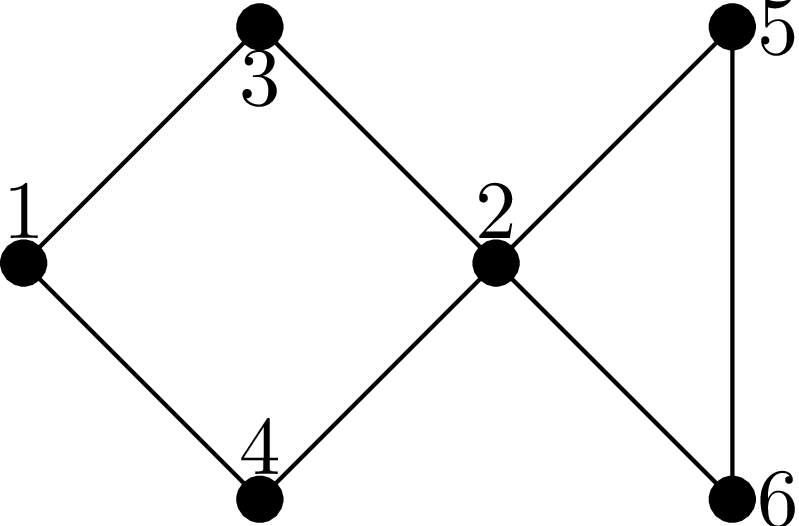
\includegraphics{texts/04_3_topsort/graph.1}\\[0.2cm]
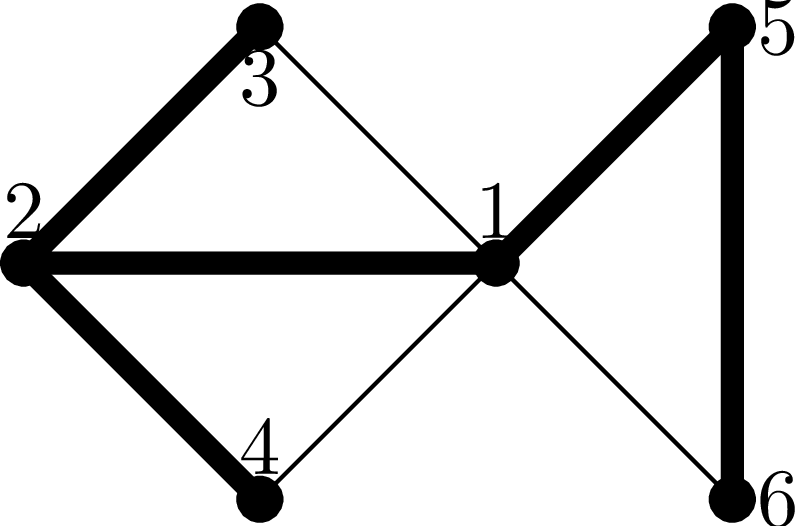
\includegraphics{texts/04_3_topsort/graph.2}
\end{wrapfigure}

Замечу, что в ациклическом графе каждая вершина является отдельной компонентой сильной связности, поскольку наличие двух
вершин в одной компоненте сильной связности очевидно обозначает наличие цикла.

Итак, поставим задачу нахождения сильносвязных компонент графа. Есть известный алгоритм их поиска. Я не знаю,
как до него можно додуматься самим и с трудом представляю, как его доказать (в Кормене есть двухстраничное 
доказательство его, которое я с большим трудом осознал), поэтому я его доказывать не буду.

Итак, алгоритм следующий. Сначала запустим алгоритм топологической сортировки поиском в глубину "--- он выдаст 
нам некоторую последовательность вершин (конечно, в случае неациклического графа она не будет решением задачи о топсорте, 
но какая"=то последовательность вершин получится). После этого сделаем следующее: запустим поиск в глубину ещё раз, но будем
двигаться по \textit{инвертированным} рёбрам, а во внешнем цикле поиска будем просматривать вершины в том порядке, 
в котором нам их выдал топсорт. Т.е. обратим направление каждого ребра графа и запустим поиск в глубину, перебирая 
во внешнем цикле вершины в этом особом порядке. (Ясно, что скорее всего вы не будете инвертировать ребра,
а просто в поиске будете писать условие типа $gr[j,i]<>0$ вместо $gr[i,j]<>0$). Утверждается, что те "<компоненты
связности">, которые вы найдёте при втором поиске, как раз и будут сильносвязными компонентами исходного графа.

\begin{codesamplec}{3}\begin{verbatim}
procedure find(i:integer);
var j:integer;
begin
if was[i]<>0 then
   exit;
was[i]:=1;
for j:=1 to n do
    if gr[i,j]<>0 then
       find(j);
ts[pos]:=i;
dec(pos);
end;

procedure find2(i:integer);
var j:integer;
begin
if was[i]<>0 then
   exit;
was[i]:=nc;
for j:=1 to n do
    if gr[j,i]<>0 then
       find2(j);
end;

...
fillchar(was,sizeof(was),0);
pos:=n;
for i:=1 to n do
    find(i);
fillchar(was,sizeof(was),0);
nc:=0;
for i:=1 to n do
    if was[ts[i]]=0 then begin
       inc(nc);
       find2(ts[i]);
    end;
\end{verbatim}
\end{codesamplec}

Ещё раз обратите внимание, как алгоритм состоит из двух частей: первые четыре строки в основном алгоритме "--- топсорт,
остальное в точности повторяет поиск обычных компонент связности в неориентированно графе. Обратите внимание, что для
них используются \textit{разные} процедуры find, поскольку, хотя обе процедуры реализуют поиск в глубину,
но они делают разные вещи в дополнение к собственно поиску. 

Ещё замечу, что тут стандартная ошибка "--- в рекурсивном вызове во второй процедуре вызвать первую, а не вторую,
 т.е. написать
\begin{codesampleo}\begin{verbatim}
procedure find2(i:integer);
...
    if gr[j,i]<>0 then
       find(j);
\end{verbatim}
\end{codesampleo}
Всегда, когда у вас в программе есть две процедуры с похожими именами, следите, чтобы их не перепутать. Особенно если эти процедуры рекурсивны "--- не перепутайте, где какую функцию в рекурсивном вызове вызывать. Даже более общее утверждение: 
если есть два похожих куска кода, особенно внимательно просмотрите, не сглючили ли вы где"=нибудь. Например, если
у вас два поиска в глубину по двум \textit{разным} графам, не перепутайте графы внутри процедур, не перепутайте рекурсивные
вызовы и т.д. Особенно это важно, если один блок вы получаете копирование из другого.

Ещё обратите внимание, что во втором поиске используется $gr[j,i]<>0$: поиск идёт в инвертированном графе.

В общем, как я уже сказал, я не знаю, как до этого алгоритма можно дойти, и не знаю, как его легко доказать. Поэтому
имхо этот алгоритм нужно примерно запомнить. Собственно, запоминать тут нечего: два поиска в глубину, причём второй
"--- в инвертированном графе. Единственное, что не очевидно, как запомнить, "--- это то, в каком порядке стоит перебирать
вершины при втором поиске в глубину. Но это легко восстанавливается: представьте себе \textit{ациклический} граф.
В нем, очевидно, каждая компонента сильной связности "--- это отдельная вершина. Очевидно, что такие компоненты
мы получим, только если будем второй поиск запускать в порядке, который мы получим из топсорта (не забудьте, что 
второй поиск "--- в инвертированном графе!). Конечно, это не очевидно, а надо представить себе ациклический 
оттопсорченный граф в уме и просто прикинуть, какие последствия будут у разных порядков выбора вершин. Если все ещё 
не понятно, то нарисуйте оттопсорченный ациклический граф и попробуйте в нем позапускать поиск в глубину в инвертированном
графе, перебирая вершины слева направо, справа налево и т.п. 

В общем, по"=моему, этот алгоритм довольно легко можно запомнить.

\task|(нетривиальное) Не очевидно, что не работает такой алгоритм: оттопсортим граф и пойдём поиском в глубину в 
\textbf{не}инвертированном графе \emph{справа налево}, т.е. от последних вершин к первым. Придумайте контрпример
к этому алгоритму (конечно, придумать контрпример проще, чем доказать корректность :) ).
||
||Пример графа, для которого такой алгоритм не работает: три вершины, ребра $1\to 3$, $3\to 1$ и $1\to 2$.
Если запустим первый поиск в глубину из вершины 1, то результат "<топсорта"> будет именно порядок 1, 2, 3, и,
пойдя в неинвертированном графе справа налево, запустившись первым же запуском $find(3)$, мы посетим все три
вершины, что неправильно. Как "<на пальцах"> объяснить, чем таким этот алгоритм отличается от верного, я не знаю.
|\label{badSCC}

\lheader{Конденсация графа}

\begin{wrapfigure}{r}{3.9cm}
\vspace{-0.3cm}
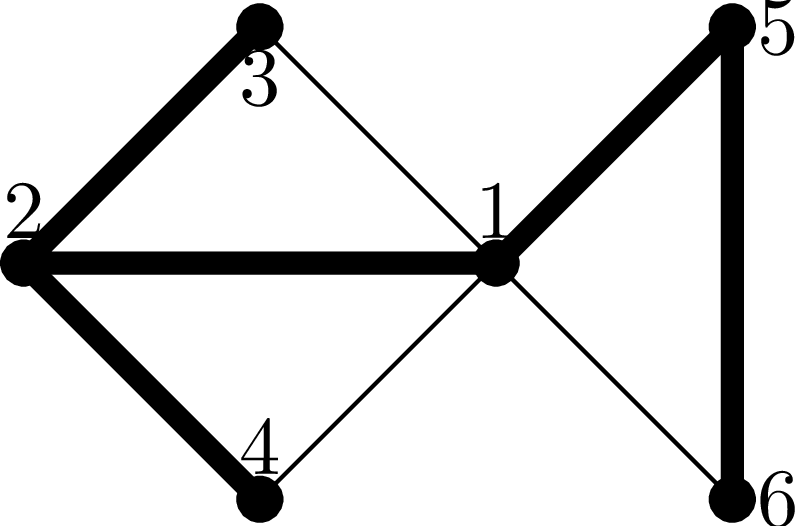
\includegraphics{texts/04_3_topsort/graph.2}\\[0.2cm]
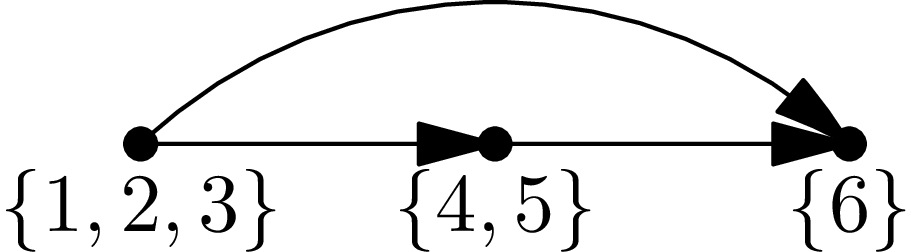
\includegraphics{texts/04_3_topsort/graph.3}
\end{wrapfigure}

Пусть у нас есть ациклический граф. Выделим в нем компоненты сильной связности и сожмём каждую в одну вершину. Т.е.
рассмотрим новый граф: в нем каждая вершина отвечает компоненте сильносвязности начального графа, ребра, шедшие между
вершинами из разных компонент, сохранены (если при этом получаются парные ребра, то оставляют только одно из них), а 
ребра, шедшие в пределах одной компоненты, не сохраняются. То, что получится, называется конденсацией этого графа. 
 
Справа приведён пример ориентированного графа с выделенными компонентами сильной связности
(то же, что и выше, в теме про компоненты сильной связности), и
его конденсации. Поскольку компонент сильной связности три, то и вершин в конденсированном графе три, 
соответствующие этим самым компонентам.

\task|Докажите, что конденсация произвольного графа является ациклическим графом.
||
||Пусть в конденсации есть цикл. Но тогда возьмём две вершины этого цикла "---
пусть это вершины 1 и 2. В конденсации по этому циклу можно дойти и из 1 в 2, и из 2 в 1. Тогда возьмём в изначальном графе 
две вершины $1'$ и $2'$ из компонент сильной связности, соответствующих вершинам 1 и 2 конденсации. Несложно показать,
что тогда и из $1'$ в $2'$ и в обратную сторону можно дойти в начальном графе, что противоречит тому,
что они лежат в разных компонентах сильной связности.
|\label{condensationisacyclic}

Как построить конденсацию графа? Ну в принципе довольно очевидно. Ищем сильносвязные компоненты, а потом строим новый 
граф (т.е. заводим новую матрицу смежности или т.п.) и добавляем в него ребра,
просто пробегаясь по рёбрам старого графа и те, которые идут в пределах одной компоненты, игнорируем, а те, которые 
идут из одной компоненты в другую, добавляем к получающемуся графу. Все просто.

В чем смысл конденсации? Ну например вот в чем. Пусть у нас есть набор объектов, про которые известно, что их можно
в каком-то смысле упорядочить, и пусть про некоторые пары объектов дано утверждение вида 
"<первый объект \textit{меньше или равен} второго"> (а про остальные пары ничего не известно). 
Ясно, что этому соответствует ориентированный граф. Несложно
понять, что компоненты сильной связности такого графа "--- это множества объектов такие, которые \textit{точно} должны
быть равны: ведь каждый из них получается меньше или равен сам себя. Тогда логично эти объекты объединить в одну вершину,
ведь они все равны между собой. Осталось определить отношения между такими "<классами">, т.е. про некоторые классы
сказать, что "<объекты одного класса меньше или равны объектов другого класса">. Если пользоваться только теми отношениями,
которые нам даны с самого начала, и не пытаться получить дополнительных следствий из них, то то что нам надо "---
это как раз и есть конденсация начального графа.

Замечу, что если бы с самого начала были даны условия вида "<один объект \textit{строго меньше} второго">, то 
граф был бы обязан быть ациклическим. Ясно, что в этом случае задача конденсации большого смысле не имеет (конденсация
ациклического графа есть сам этот граф, т.к. каждая компонента сильной связности тут состоит из одной вершины), но может
иметь смысл задача поиска какого"=нибудь порядка объектов, не противоречащего этим условиям "--- а это делает топсорт.

Ещё замечу, что можно поставить задачу так: базируясь на данных нам условиях об объектах, перечислить 
\textit{наибольшее} возможное количество пар объектов, про которые мы можем сделать аналогичное утверждение.
Здесь придётся пользоваться транзитивностью отношения "<меньше"> (или "<меньше или равно">, в зависимости от того,
какие условия нам даны): т.е. тем, что, если $a<b$, а $b<c$, то $a<c$. Т.е., если нам даны условия
$$
a<b,\quad b<c,\quad b<d,
$$
то мы должны сказать, что $a<b$, $a<c$, $a<d$, $b<c$, $b<d$, но про $c$ и $d$ ничего сказать не можем. Такая задача
называется \textit{транзитивным замыканием графа}, она не решается ни одним из рассмотренных выше алгоритмов, для
неё есть отдельный алгоритм, про который мы поговорим как"=нибудь в другой раз "--- к поиску в глубину он имеет
мало отношения.

\lheader{Времена входа и выхода}
Очень часто при обсуждении поиска в глубину вводят такие понятия, как времена входа и выхода. А именно, заведём 
глобальный счётчик "<времени"> $t$ и каждый раз, когда мы первый раз начинаем обработку очередной вершины (входим
в неё), и каждый раз, когда заканчиваем обработку вершины (выходим из неё) будем увеличивать $t$ на единицу, а 
полученное значение записывать как "<время входа"> или "<время выхода"> в/из этой вершины, соответственно.
Т.е. получим следующий алгоритм:
\begin{codesample}\begin{verbatim}
procedure find(i:integer);
begin
if was[i]<>0 then
   exit;
was[i]:=1;
inc(t);
s[i]:=t;
for i:=1 to n do
    if gr[i,j]=1 then
       find(j);
inc(t);
f[i]:=t;
end;


...
fillchar(was,sizeof(was),0);
t:=0;
for i:=1 to n do
    find(i);





\end{verbatim}
\end{codesample}
Здесь $s$ "--- массив времён входа (т.е. $s[i]$ "--- время входа в $i$-ю вершину), а $f$ "--- аналогичный массив времён выхода. Перед запуском поиска в глубину занулим переменную $t$. 

Обратите ещё раз внимание, что при работе этого 
алгоритма каждый элемент массива $s$ будет установлен \textit{ровно} один раз (т.е. каждый элемент будет установлен:
не будет вершин, у которых время входа останется неопределённым "--- и никакой элемент не будет переписываться:
не будет такого, что мы сначала в $s[i]$ запишем одно значение, а потом туда же другое), поскольку
каждую вершину мы обрабатываем ровно один раз. Аналогично с массивом $f$.

Ещё обратите внимание, что массив $was$ теперь не нужен, вместо него можно использовать массив $s$ (но не $f$!),
только, конечно, тогда $s$ нужно будет предварительно занулить. Или, что то же самое, времена входа можно хранить 
в массиве $was$, а не в $s$ (как раньше мы номер компоненты связности хранили в $was$). Здесь я использую
$s$ только для наглядности.

Но в реальных задачах времена входа и выхода, как правило, не бывают нужны. Они часто помогают в теоретических 
рассуждениях, но реально их вычислять обычно не нужно; более того, как мне кажется, нередко понять алгоритм проще, если 
не обращаться к понятию времён входа/входа. Например, часто при описании алгоритмов употребляется фраза 
"<отсортируем вершины по временам выхода"> (реже по временах входа), но это не значит, что нужно вычислять эти 
времена, а потом писать QSort или что"=нибудь подобное. Все делается намного проще.
                      
\task|Как надо правильно и проще всего сортировать вершины по временам выхода? Аналогично по временам входа.
||Подумайте, что же, собственно, делает алгоритм топологической сортировки в плане времён выхода?
||Несложно видеть, что топсорт как раз и сортирует вершины по времени выхода, только
в порядке убывания. Он ведь на последнее место в выходном массиве ставит вершину, из которой мы вышли первой, 
и т.д. Поэтому сортировать вершины по времени выхода надо аналогично топсорту. По времени входа сортировать
тоже аналогично, только ставить вершину в выходной массив надо в начале процедуры $find$. Это чем-то аналогично
сортировке подсчётом.
|\label{howtosort}

Обязательно прочитайте ответ к этой задаче! (Конечно, только после того, как порешаете сами).
